\section{Experimentación}

Dada la cantidad de vértices, los grafos se generan en el formato estándar DIMACS \footnote{Para ver algunos ejemplos del formato: http://mat.gsia.cmu.edu/COLOR/instances.html}. El generador toma como parámetro la densidad del grafo. Dada una clique con esa cantidad de vértices, se elijen vértices al azar hasta que se llega a la densidad deseada. Debido a que estas instancias están diseñadas para coloreo de grafos, asignamos los vértices de forma uniforme en el total de particiones pasado por parámetro a nuestro programa de coloreo particionado.

Por cuestiones de tiempo, cada uno de los experimientos CPLEX fue ejecutado sin límite de cantidad de threads, con un procesador Intel(R) Core(TM) i7-3610QM CPU @ 2.30GHz y 16GB de memoria RAM.

\subsection{Eliminación de simetría}

Al igual que el problema de coloreo de grafos, el problema del coloreo particionado de grafos presenta una gran cantidad de soluciones simétricas. De no romper la simetría del problema, los algoritmos tendrían un espacio de búsqueda mucho mayor, moviéndose por soluciones que, siendo computacionalmente distintas, en la práctica se trata de la misma. Esto afecta el tiempo de ejecución de forma considerable a medida que crece el tamaño del problema. Para romper la simetría en nuestro problema, en la sección \ref{simetria} mostramos cómo utilizamos la clásica condicion de coloreo de que los colores se deben utilizar en orden. Este fenómeno se puede ver en el siguiente gráfico:

\begin{figure}[h]
\centering
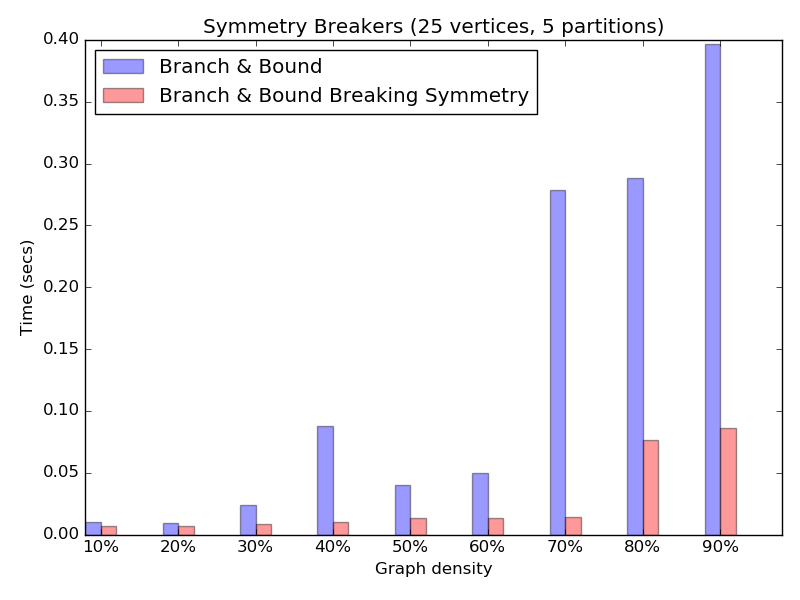
\includegraphics[scale=0.7]{img/2-symmetry_v25_p5_l40_t1_b0.png}
\caption{Tiempo de resolución del modelo incluyendo o no eliminación de simetría.}
\end{figure}

Esto nos brinda la noción de la importancia y efectividad de romper simetría al realizar la formulación de un LP. Cabe mencionar que existen muchas otras estrategias o expresiones para disminuir aun más el grado de simetría de la formulación. La formulación elegida no debe ser considerada necesarimante la mejor posible.

\pagebreak

\subsection{Efectividad de las familias de desigualdades}

La idea de este experimento es comparar las diferentes estrategias de planos de corte. Para ello, se eligió a 40 como la cantidad de cortes de cada tipo que se podían agregar, con una sola iteración:

\begin{figure}[h]
  \centering
  \begin{minipage}[b]{0.49\textwidth}
    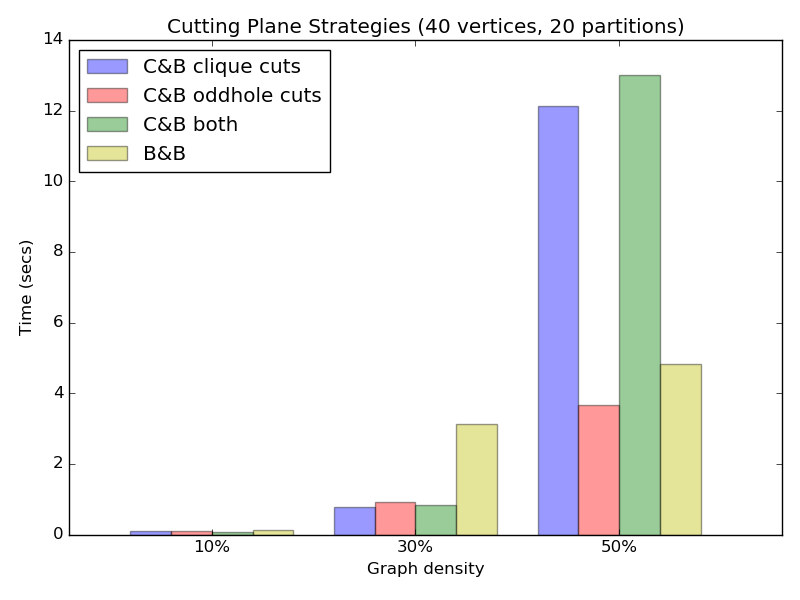
\includegraphics[width=\textwidth]{img/5-cuts_v40_p20_i1_l40_t1_b0.png}
    \caption{Estrategias de planos de corte (tiempo).}
  \end{minipage}
  \hfill
  \begin{minipage}[b]{0.49\textwidth}
    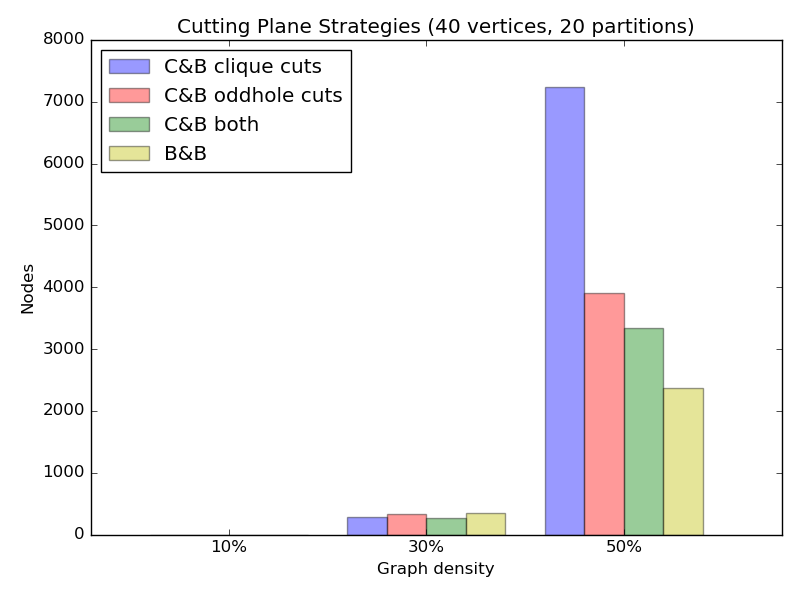
\includegraphics[width=\textwidth]{img/5-cuts_v40_p20_i1_l40_t1_b0_nodes.png}
    \caption{Estrategias de planos de corte (nodos).}
  \end{minipage}
\end{figure}

Lo primero que podemos observar es que no siempre hay una estrategia ganadora por sobre las otras. Al aumentar la densidad del grafo, pueden más distinguidamente los distintos métodos.

En el caso de los grafos más densos, uno esperaría a priori que nuestra heurística encuentre más cliques, y que los tiempos sean mejores. Esto no sucede, y de hecho, agregar las restriciones de clique empeora el tiempo de ejecución con respecto a utilizar simplemente B\&B. En los grafos menos densos, puede notarse un efecto positivo de los cortes, es decir preferencia del C\&B sobre el B\&B.

En contra de lo que esperábamos inicialmente, las desigualdades de agujero impar parecen funcionar bien, realizando mejores tiempos que el B\&B. Sin embargo, esta hipótesis podría constatarse con mayor peso de llevar a cabo una experimentación más exhaustiva.

Por último, también podemos observar que un mejor tiempo de ejecución no necesariamente implica que se recorren menos nodos del árbol. Esto puede ser interesante tenerlo en cuenta en el caso de que uno compare en qué lugar se consume el tiempo de ejecución, o para evaluar distintas formas de poda del árbol.

\subsection{Efecto de aumentar el número de particiones}

\begin{figure}[h]
  \centering
  \begin{minipage}[b]{0.49\textwidth}
    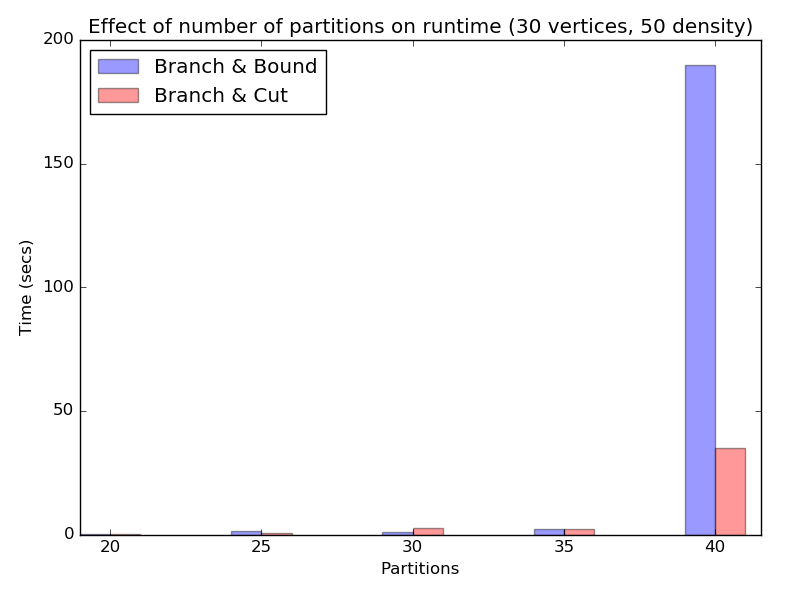
\includegraphics[width=\textwidth]{img/3-partitions_v30_d50_i1_co0_l40_t1_b0.png}
    \caption{Tiempo de ejecucion a medida que aumenta el número de particiones.}
  \end{minipage}
  \hfill
  \begin{minipage}[b]{0.49\textwidth}
    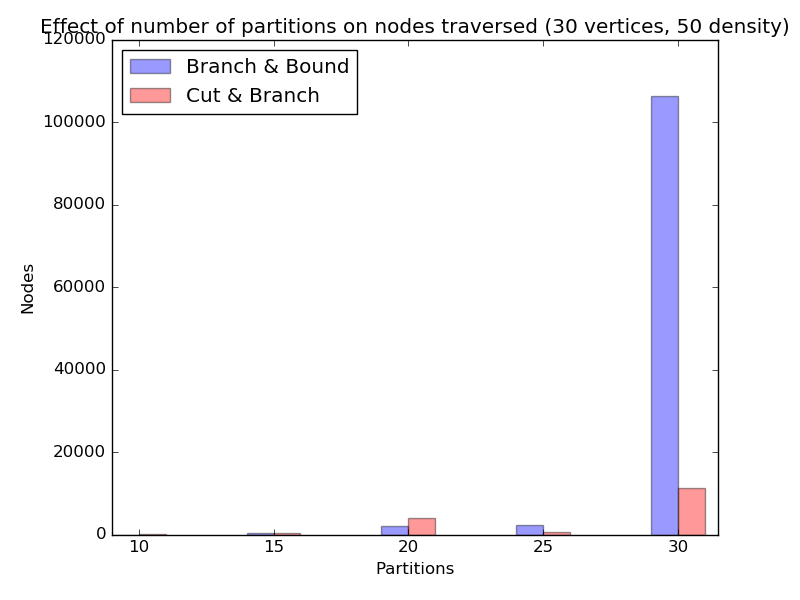
\includegraphics[width=\textwidth]{img/3-partitions_v30_d50_i1_co0_l40_t1_b0_nodes.png}
    \caption{Nodos recorridos a medida que aumenta el número de particiones.}
  \end{minipage}
\end{figure}

A medida que aumentamos el número de particiones, el problema comienza a parecerse más a uno de coloreo. Dado que las desigualdades que implementamos son clásicas de coloreo, es de esperar que la performance mejore a medida que aumenta el número de particiones. Para Cut \& Branch, sólo utilizamos los mejores 40 cortes de clique con una iteración. A medida que aumenta el número de particiones, podemos observar que el efecto positivo de incluir los cortes es considerable.

En cuanto a los nodos recorridos, puede verse que en el caso del C\&B la cantidad es notablemente menor. Se atribuye esto a la virtud de los cortes de generar una buena solución al inicio, permitiendo descartar ramas del árbol.

\subsection{Efecto de aumentar la densidad del grafo}

\begin{figure}[h]
  \centering
  \begin{minipage}[b]{0.49\textwidth}
    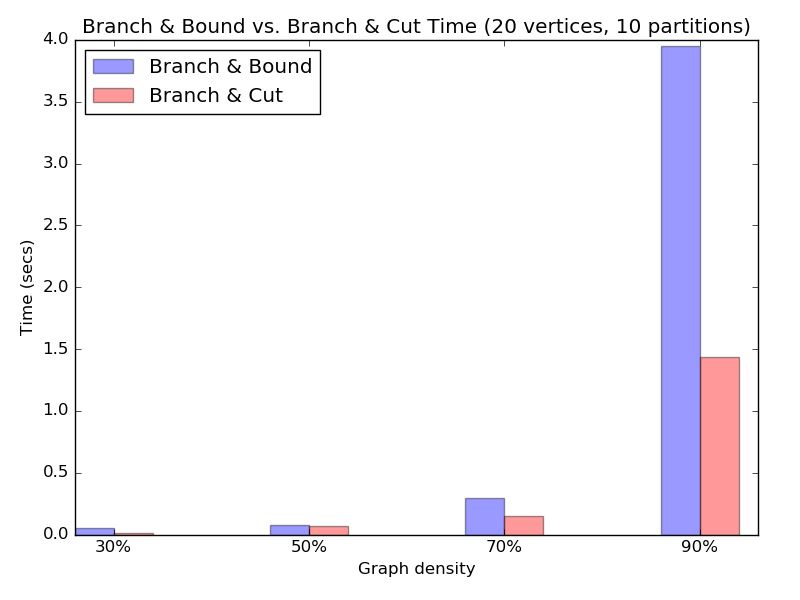
\includegraphics[width=\textwidth]{img/1-bb_vs_bc_v20_p10_i1_co0_l40_t1_b0.png}
  \end{minipage}
  \hfill
  \begin{minipage}[b]{0.49\textwidth}
    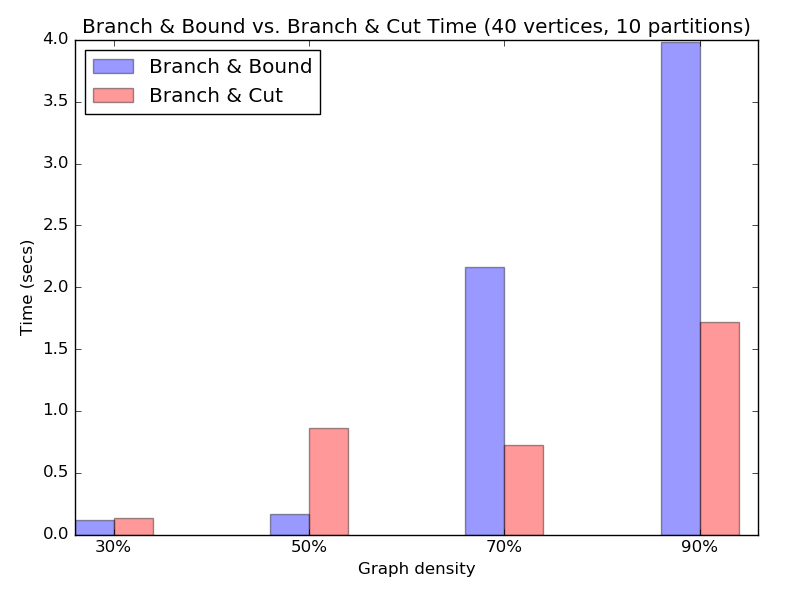
\includegraphics[width=\textwidth]{img/1-bb_vs_bc_v40_p10_i1_co0_l40_t1_b0.png}
  \end{minipage}
  \begin{minipage}[b]{0.49\textwidth}
    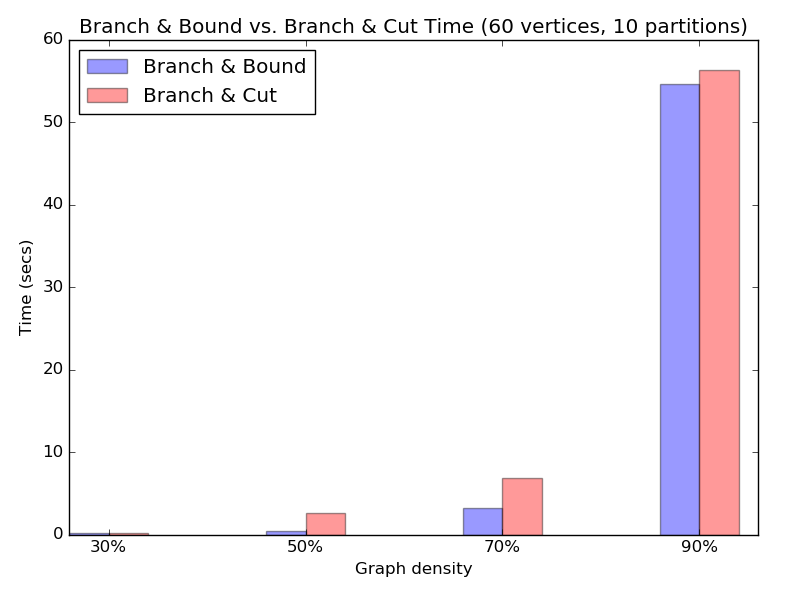
\includegraphics[width=\textwidth]{img/1-bb_vs_bc_v60_p10_i1_co0_l40_t1_b0.png}
  \end{minipage}
  \hfill
  \begin{minipage}[b]{0.49\textwidth}
    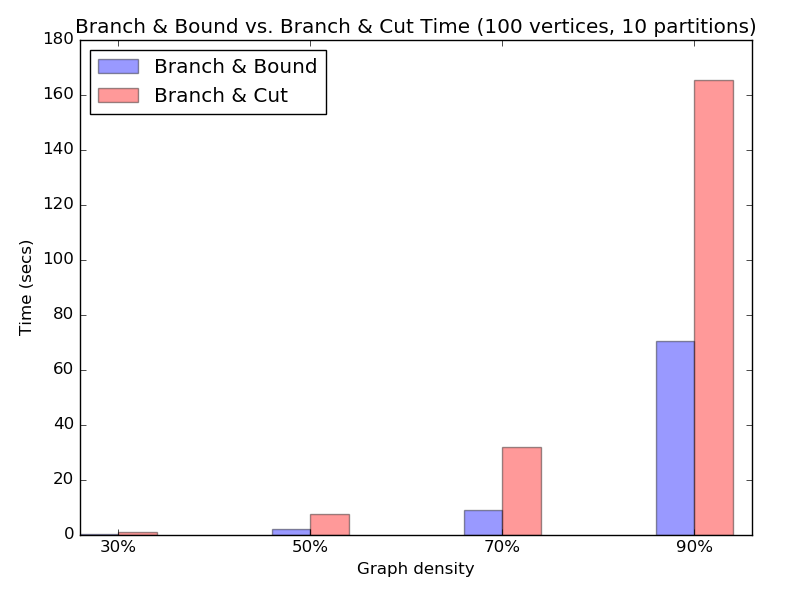
\includegraphics[width=\textwidth]{img/1-bb_vs_bc_v100_p10_i1_co0_l40_t1_b0.png}
  \end{minipage}
	\caption{Efecto de aumentar la densidad del grafo.}
\end{figure}

A medida que aumenta la densidad del grafo, el problema de coloreo se vuelve sin duda más difícil. En gráficos más densos y cuya relación de número de particiones sobre número de vértices es mayor se puede apreciar una tendencia a funcionar mejor del Branch \& Cut (nuevamente se utiliza 1 iteración y 40 desigualdades violadas). Sin embargo, en grafos esparsos, podemos notar una mayor efectividad del Branch \& Bound puro, en cuanto a tiempos de ejecución. De cualquier modo, no es posible obtener resultados muy generales, sino más bien mejores o peores algoritmos para cierta densidad y cantidad de particiones.

\subsection{Efecto de aumentar la cantidad de restricciones incorporadas por iteración}

Para todos nuestros experimentos en general utilizamos sólo 1 iteración con un límite de 40 desigualdades por familia. La idea de este experimento es evaluar esta configuración. Para ello, utilizamos un grafo con 40 vértices y 20 particiones.

\begin{figure}[h]
  \centering
  \begin{minipage}[b]{0.49\textwidth}
    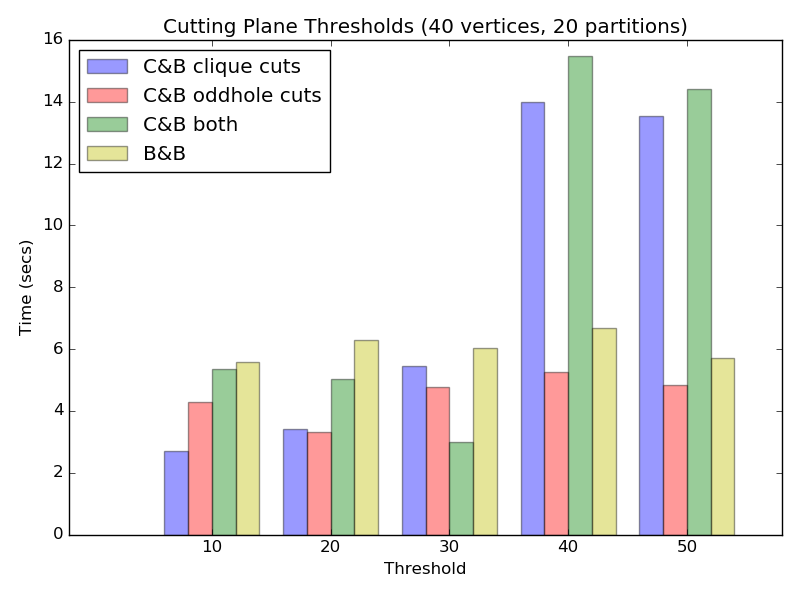
\includegraphics[width=\textwidth]{img/6-thresholds_v40_p20_i1_t1_b0.png}
    \caption{Tiempo de ejecución al incrementar el número de restricciones incorporadas.}
  \end{minipage}
  \hfill
  \begin{minipage}[b]{0.49\textwidth}
    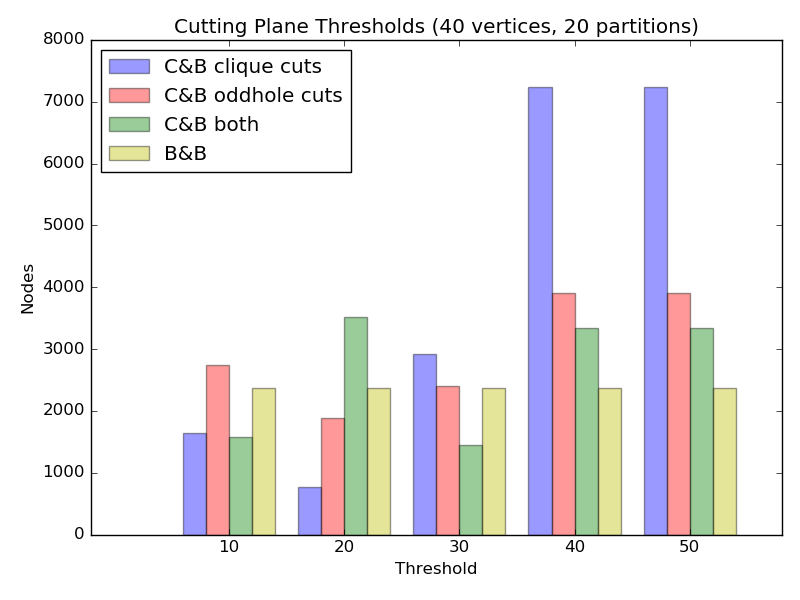
\includegraphics[width=\textwidth]{img/6-thresholds_v40_p20_i1_co2_t1_b0_nodes.png}
    \caption{Nodos recorridos al incrementar el número de restricciones incorporadas.}
  \end{minipage}
\end{figure}

Como podemos concluirse de los gráficos, agregar más restricciones no es siempre ventajoso. En un principio, sumar restricciones parece mejorar la ejecución del C\&B (para el caso de ambas familias), pero ya a partir de las 40 el tiempo de ejecución empeora de forma abrupta para las cliques. Esto no sucede para las restricciones de agujero impar, cuyo tiempo de ejecución no posee gran variabilidad con respecto al $threshold$.

Claro está, que este incremento en el tiempo puede estar relacionado con la heurística de clique utilizada, que puede no se lo suficientemente buena. Debido al saldo importante que ocurre con los cortes por cliques, el $threshold$ de 30 se considera empíricamente aceptable.

Por otro lado, es visible en el primer gráfico una dependencia del tiempo de ejecución del B\&B con respecto al $threshold$ analizado. Sabemos que esta variabilidad no corresponde, y se atribuye a ruido del CPU.

\subsection{Efecto de aumentar la cantidad de iteraciones de planos de corte}

\begin{figure}[h]
\centering
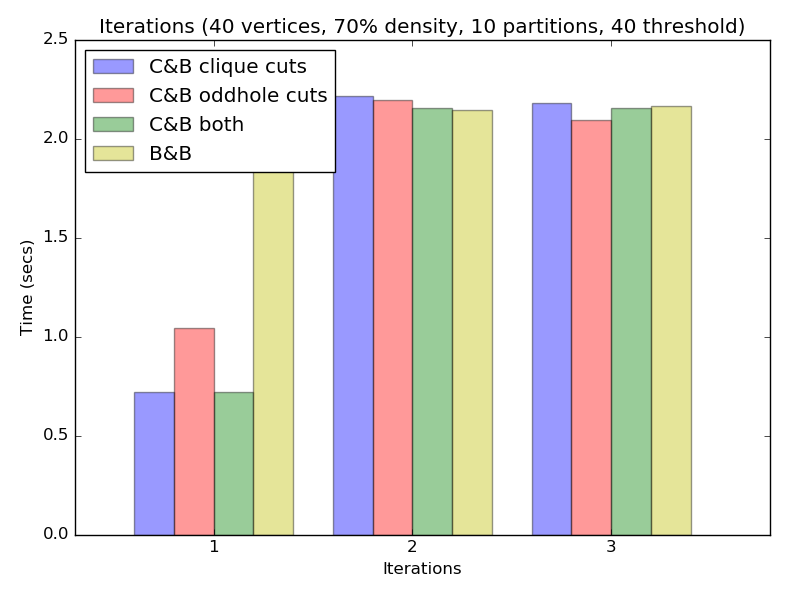
\includegraphics[scale=0.5]{img/7-iterations_v40_p10_l40_t1_b0.png}
\caption{Tiempo de ejecución al aumentar la cantidad de iteraciones de planos de corte.}
\end{figure}

Como podemos ver, aumentar el número de iteraciones de planos de corte no necesariamente mejora el tiempo de ejecución. En cada iteración, lo que hacíamos era generar una familia de desigualdades en función de la solución de la relajación del problema, y luego agregar las \textit{mejores} restricciones. En relación con la sección anterior, también está relacionado con el $threshold$ elegido para la experimentación.

\pagebreak

\subsection{Comparación B\&B, C\&B, CPLEX default}

\begin{figure}[h]
  \centering
  \begin{minipage}[b]{0.49\textwidth}
    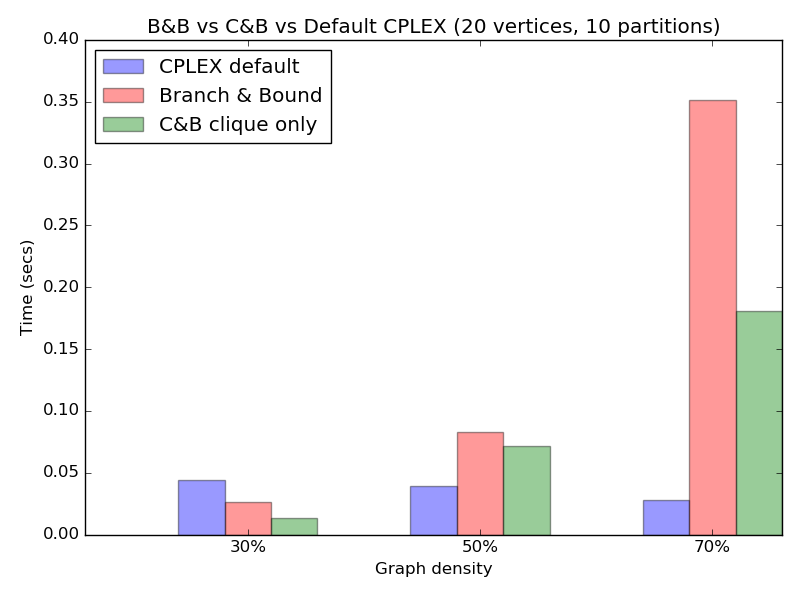
\includegraphics[width=\textwidth]{img/8-compare_v20_p10_i1_l40_t1_b0.png}
  \end{minipage}
  \hfill
  \begin{minipage}[b]{0.49\textwidth}
    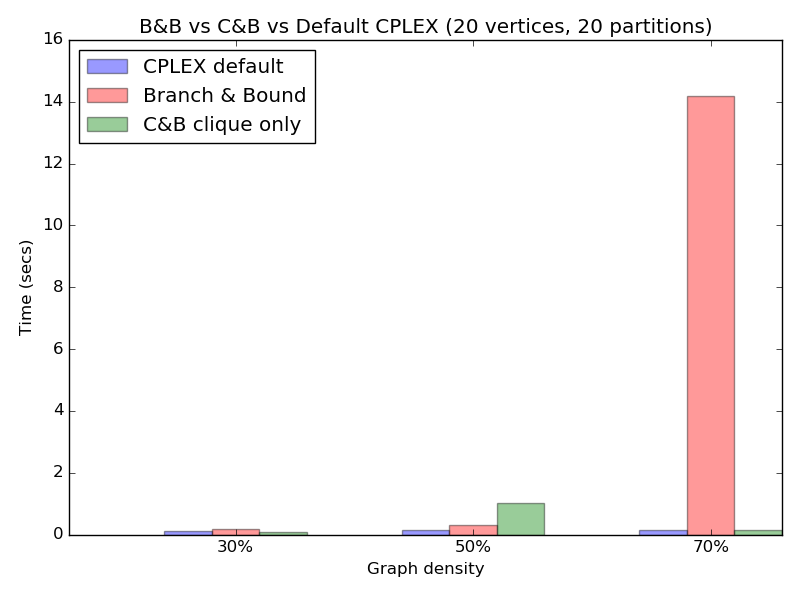
\includegraphics[width=\textwidth]{img/8-compare_v20_p20_i1_l40_t1_b0.png}
  \end{minipage}
  \begin{minipage}[b]{0.49\textwidth}
    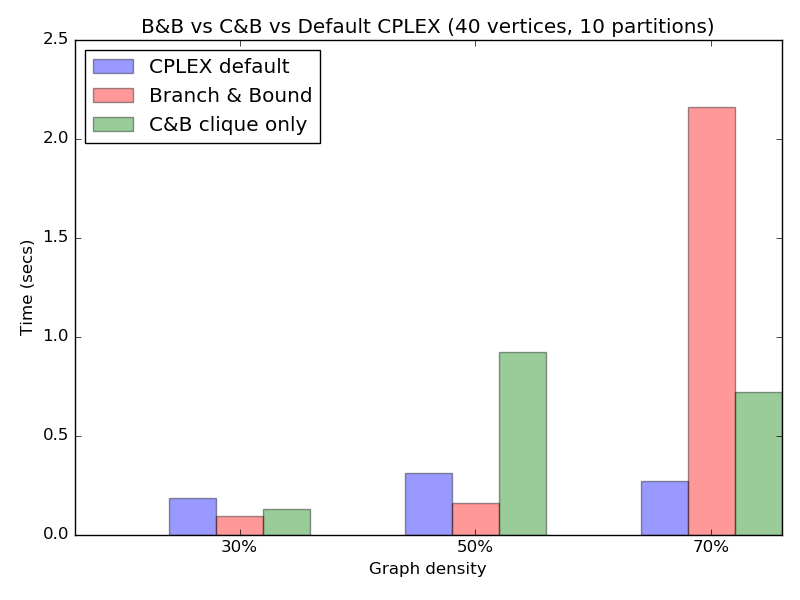
\includegraphics[width=\textwidth]{img/8-compare_v40_p10_i1_l40_t1_b0.png}
  \end{minipage}
  \hfill
  \begin{minipage}[b]{0.49\textwidth}
    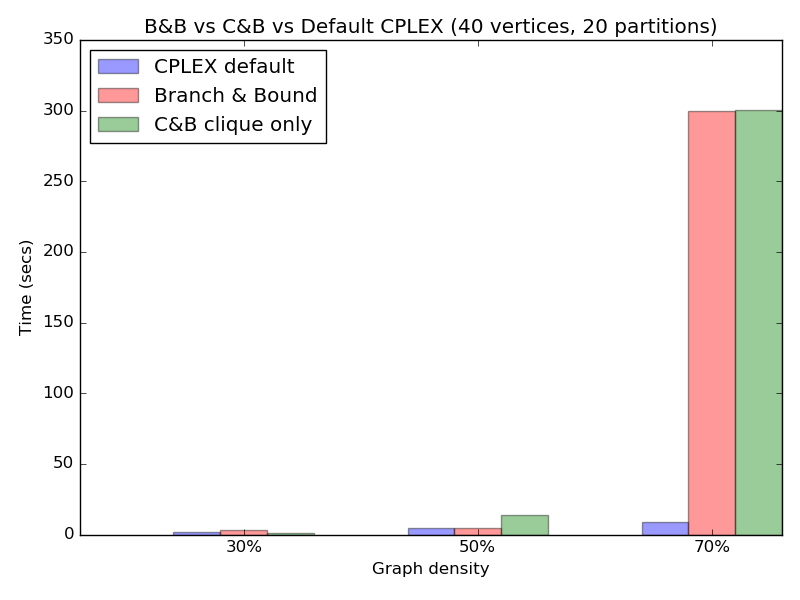
\includegraphics[width=\textwidth]{img/8-compare_v40_p20_i1_l40_t1_b0.png}
  \end{minipage}
	\caption{Comparacion B\&B, C\&B, CPLEX default para diferentes grafos.}
\end{figure}

Dado que el CPLEX utiliza por default cortes de Gomory y preprocesamiento de variables, no nos sorprende que en general para grafos densos sea notablemente superior. Una propuesta interesante podría ser repetir esta experimentación permitiendo los cortes y el preprocesamiento para todas nuestras estrategias.

Al mismo tiempo, es importante observar el gráfico superior derecho, que corresponde al coloreo de grafos estándar (cada vértice pertenece a una partición diferente). En él se puede apreciar la gran utilidad de las desigualdades de clique para disminuir tiempos de ejecución, en el caso de grafos densos. 

\subsection{Estrategias de recorrido del árbol de enumeración
y selección de variable de branching}

Existen muchas estrategias de recorrido del árbol de enumeración. En este trabajo analizaremos únicamente Depth First Search (DFS) y Best Bound Search (BBS). DFS recorre el árbol de enumeración de B\&B primero en profundidad, mientras que BBS recorre el árbol de enumeración buscando una buena cota lo más rápido posible, de modo de realizar una buena poda. En general, se utilizan estrategias heurísticas. En el caso de CPLEX, dado un nodo padre se calcula la solución a la relajación de todos sus hijos y luego se continua recorriendo el nodo con el mayor resultado de la función objetivo. \footnote{http://www-01.ibm.com/support/knowledgecenter/SSSA5P\_12.6.1/ilog.odms.cplex.help/CPLEX/Parameters/topics/NodeSel.html}.

Ambas estrategias son sumamente ventajosas, ya que permiten obtener una cota superior a la solución final para utilizar de poda al hacer backtracking sobre el árbol de enumeración. Dado que no utilizamos heurísticas iniciales, esta estrategia parece razonable. 

Por otro lado, las estrategias de selección de variable buscan encontrar cuál es la mejor variable sobre la que hacer branching. Hay muchas reglas, como por ejemplo \textit{max/min infeasibility}. Mientras que la regla de \textit{minimum infeasibility} hace branching sobre aquella variable más cercana al valor entero, la regla de \textit{maximum infeasibility} hace exactamente lo contrario \footnote{http://www-01.ibm.com/support/knowledgecenter/SS9UKU\_12.4.0/com.ibm.cplex.zos.help/Parameters/topics/VarSel.html}.

En esta sección analizaremos 4 combinaciones de estrategias de recorrido del árbol de enumeración y selección de variable de branching para B\&B puro y C\&B con cortes de clique, 1 iteración y $threshold$ 30. Las combinaciones que analizaremos son DFS + MAXINFEAS, DFS + MININFEAS, BESTBOUND + MAXINFEAS y BESTBOUND + MININFEAS.

\begin{figure}[h]
  \centering
  \begin{minipage}[b]{0.49\textwidth}
    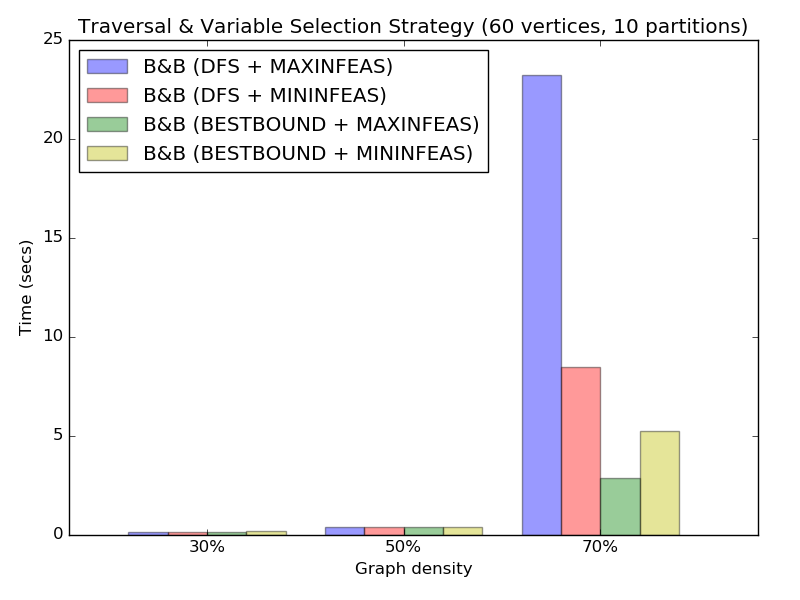
\includegraphics[width=\textwidth]{img/9-tree_v60_p10_i1_l30_s1.png}
  \end{minipage}
  \hfill
  \begin{minipage}[b]{0.49\textwidth}
    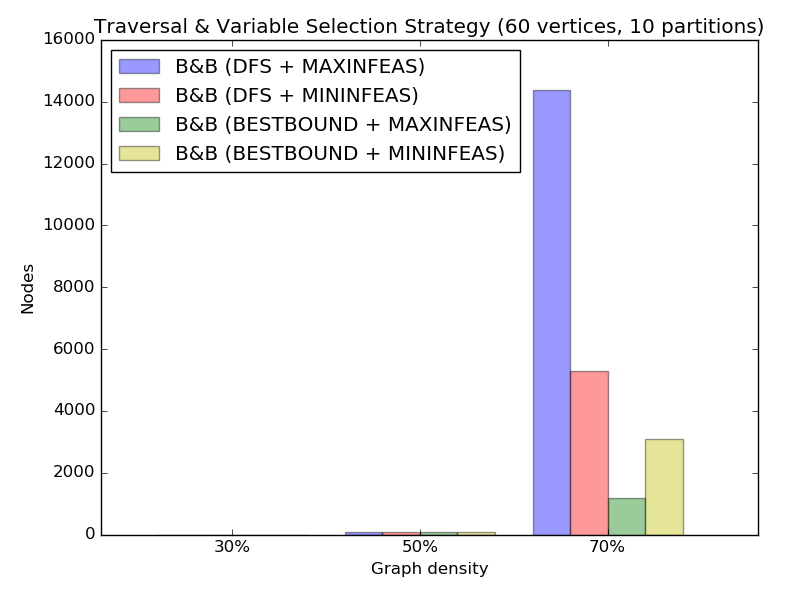
\includegraphics[width=\textwidth]{img/9-tree_v60_p10_i1_l30_s1_nodes.png}
  \end{minipage}
  \begin{minipage}[b]{0.49\textwidth}
    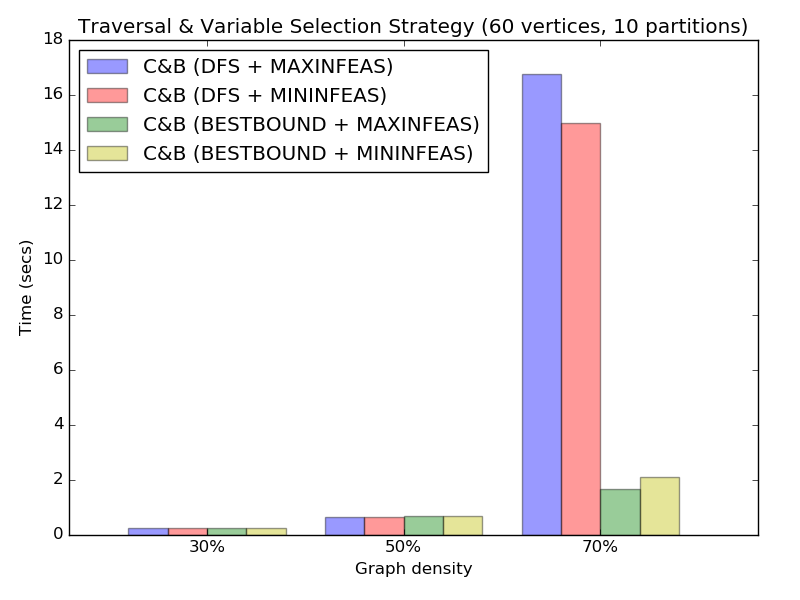
\includegraphics[width=\textwidth]{img/9-tree_v60_p10_i1_l30_s2.png}
  \caption{Tiempo de ejecución dependiendo de la estrategias de recorrido y selección de variable.}
  \end{minipage}
  \hfill
  \begin{minipage}[b]{0.49\textwidth}
    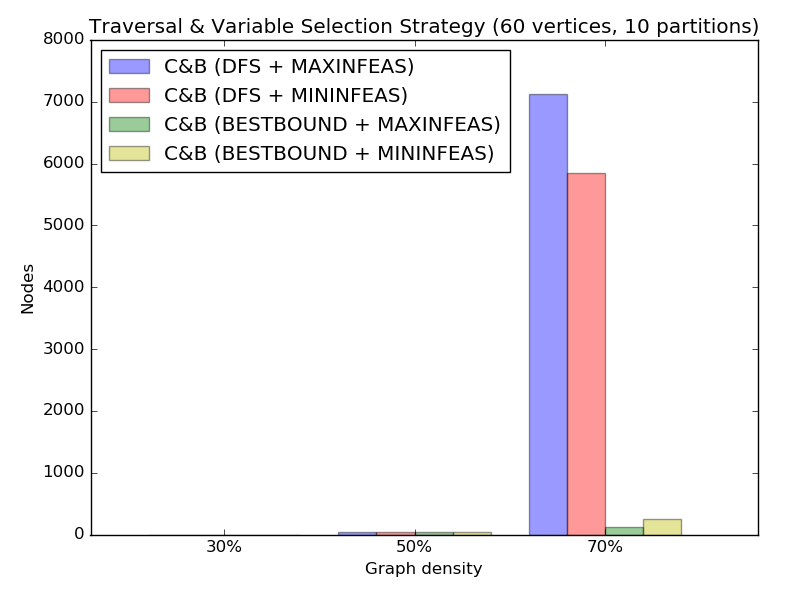
\includegraphics[width=\textwidth]{img/9-tree_v60_p10_i1_l30_s2_nodes.png}
  \caption{Nodos recorridos dependiendo de la estrategias de recorrido y selección de variable.}
  \end{minipage}
\end{figure}

Como podemos observar, en general C\&B tiene menores tiempos de ejecución, y recorre menos nodos. Al mismo tiempo, de las 4 combinaciones testeadas, la mejor estrategia para este problema parece ser BESTBOUND + MAXINFEAS. CPLEX utiliza por default BESTBOUND, aunque recurre a una heurística para elegir la variable de branching. 

\subsection{Instancias DIMACS}

Las instancias DIMACS son comúnmente utilizadas en la literatura como instancias de benchmarking. A continuación se muestran nuestros tiempos de ejecución con B\&B y B\&C utilizando 1 iteración y $threshold$ 30, utilizando sólo desigualdades de clique. La regla utilizada para recorrer el árbol de enumeración es la que utiliza el CPLEX por default.

Cada tabla utiliza fue elaborada utilizando un número de particiones diferente. Dado que las instancias DIMACS no tienen asocidas un número de partición (éstas se utilizan comúnmente para coloreo estándar), asignamos uno nosotros, y luego dividimos los vértices en orden en las diferentes particiones de forma uniforme.

Tomamos como tiempo límite de ejecución 10 minutos, y reportamos el número de colores encontrado por B\&B hasta ese momento. En todos los casos, B\&B y B\&C coincidieron con el número de colores, por lo que los reportamos en una única columna.

En este punto, quizás sería interesante probar con otras configuraciones de C\&B para los problemas más difíciles. Para esos problemas, C\&B parece mostrar una mejor performance.

\begin{table}[H]
\centering
\caption{Benchmark con 10 particiones.}
\begin{tabular}{|l|r|r|r|r|c|}
\hline
Problema & \multicolumn{1}{l|}{n} & \multicolumn{1}{l|}{m} & \multicolumn{1}{l|}{Tiempo B\&B (secs)} & \multicolumn{1}{l|}{Tiempo B\&C (secs)} & \multicolumn{1}{l|}{Colores utilizados} \\ \hline
anna & 138 & 493 & 0.04 & 0.50 & 1 \\ \hline
david & 87 & 406 & 0.02 & 0.29 & 1 \\ \hline
fpsol2.i.1 & 496 & 11654 & 0.51 & 8.71 & 1 \\ \hline
fpsol2.i.2 & 451 & 8691 & 0.44 & 7.66 & 1 \\ \hline
fpsol2.i.3 & 425 & 8688 & 0.45 & 8.15 & 1 \\ \hline
games120 & 120 & 638 & 0.04 & 0.32 & 1 \\ \hline
homer & 561 & 1629 & 0.11 & 0.72 & 1 \\ \hline
huck & 74 & 301 & 0.02 & 0.10 & 1 \\ \hline
inithx.i.1 & 864 & 18707 & 0.79 & 9.66 & 1 \\ \hline
inithx.i.2 & 645 & 13979 & 0.59 & 6.53 & 1 \\ \hline
inithx.i.3 & 621 & 13969 & 0.59 & 6.16 & 1 \\ \hline
jean & 80 & 254 & 0.02 & 0.10 & 1 \\ \hline
le450\_15a & 450 & 8168 & 0.31 & 14.68 & 1 \\ \hline
le450\_15b & 450 & 8169 & 0.35 & 15.68 & 1 \\ \hline
le450\_15c & 450 & 16680 & 0.64 & 36.05 & 1 \\ \hline
le450\_15d & 450 & 16750 & 0.83 & 38.00 & 1 \\ \hline
le450\_25a & 450 & 8260 & 0.34 & 24.95 & 1 \\ \hline
le450\_25b & 450 & 8263 & 0.33 & 15.41 & 1 \\ \hline
le450\_25c & 450 & 17343 & 0.70 & 42.17 & 1 \\ \hline
le450\_25d & 450 & 17425 & 0.70 & 39.60 & 1 \\ \hline
le450\_5a & 450 & 5714 & 0.27 & 8.19 & 1 \\ \hline
le450\_5b & 450 & 5734 & 0.30 & 13.78 & 1 \\ \hline
le450\_5c & 450 & 9803 & 0.46 & 29.12 & 1 \\ \hline
le450\_5d & 450 & 9757 & 0.47 & 33.13 & 1 \\ \hline
miles1000 & 128 & 3216 & 8.81 & 7.77 & 2 \\ \hline
miles1500 & 128 & 5198 & 600.00 & 600.00 & 3 \\ \hline
miles250 & 128 & 387 & 0.03 & 0.24 & 1 \\ \hline
miles500 & 128 & 1170 & 0.06 & 0.54 & 1 \\ \hline
miles750 & 128 & 2113 & 0.32 & 2.73 & 1 \\ \hline
mulsol.i.1 & 197 & 3925 & 0.15 & 2.20 & 1 \\ \hline
mulsol.i.2 & 188 & 3885 & 0.14 & 2.01 & 1 \\ \hline
mulsol.i.3 & 184 & 3916 & 0.16 & 3.02 & 1 \\ \hline
mulsol.i.4 & 185 & 3946 & 0.15 & 4.37 & 1 \\ \hline
mulsol.i.5 & 186 & 3973 & 0.15 & 3.42 & 1 \\ \hline
myciel3 & 11 & 20 & 0.01 & 0.01 & 3 \\ \hline
myciel4 & 23 & 71 & 0.01 & 0.02 & 1 \\ \hline
myciel5 & 47 & 236 & 0.01 & 0.04 & 1 \\ \hline
myciel6 & 95 & 755 & 0.04 & 0.29 & 1 \\ \hline
myciel7 & 191 & 2360 & 0.09 & 1.75 & 1 \\ \hline
queen10\_10 & 100 & 1470 & 0.12 & 0.61 & 1 \\ \hline
queen11\_11 & 121 & 1980 & 0.18 & 1.03 & 1 \\ \hline
queen12\_12 & 144 & 2596 & 0.36 & 2.29 & 1 \\ \hline
queen13\_13 & 169 & 3328 & 0.44 & 2.73 & 1 \\ \hline
queen14\_14 & 196 & 4186 & 0.18 & 5.05 & 1 \\ \hline
queen15\_15 & 225 & 5180 & 0.23 & 7.02 & 1 \\ \hline
queen16\_16 & 256 & 6320 & 0.23 & 8.62 & 1 \\ \hline
queen5\_5 & 25 & 160 & 0.06 & 0.14 & 3 \\ \hline
queen6\_6 & 36 & 290 & 0.12 & 0.54 & 2 \\ \hline
queen7\_7 & 49 & 476 & 0.12 & 0.41 & 2 \\ \hline
queen8\_12 & 96 & 1368 & 3.54 & 3.96 & 2 \\ \hline
queen8\_8 & 64 & 728 & 0.26 & 0.64 & 2 \\ \hline
queen9\_9 & 81 & 1056 & 1.76 & 2.54 & 2 \\ \hline
school1 & 385 & 19095 & 1.17 & 90.04 & 1 \\ \hline
school1\_nsh & 352 & 14612 & 0.83 & 46.13 & 1 \\ \hline
zeroin.i.1 & 211 & 4100 & 0.16 & 4.87 & 1 \\ \hline
zeroin.i.2 & 211 & 3541 & 0.17 & 3.82 & 1 \\ \hline
zeroin.i.3 & 206 & 3540 & 0.25 & 1.91 & 1 \\ \hline
\end{tabular}
\end{table}

\begin{table}[H]
\centering
\caption{Benchmark con 20 particiones.}
\begin{tabular}{|l|r|r|r|r|c|}
\hline
Problema & \multicolumn{1}{l|}{n} & \multicolumn{1}{l|}{m} & \multicolumn{1}{l|}{Tiempo B\&B (secs)} & \multicolumn{1}{l|}{Tiempo B\&C (secs)} & \multicolumn{1}{l|}{Colores utilizados} \\ \hline
anna & 138 & 493 & 0.07 & 0.49 & 1 \\ \hline
david & 87 & 406 & 0.04 & 0.42 & 1 \\ \hline
fpsol2.i.1 & 496 & 11654 & 1.10 & 34.07 & 1 \\ \hline
fpsol2.i.2 & 451 & 8691 & 0.75 & 17.08 & 1 \\ \hline
fpsol2.i.3 & 425 & 8688 & 0.83 & 17.88 & 1 \\ \hline
games120 & 120 & 638 & 1.85 & 2.00 & 1 \\ \hline
homer & 561 & 1629 & 0.39 & 2.35 & 1 \\ \hline
huck & 74 & 301 & 0.08 & 0.18 & 1 \\ \hline
inithx.i.1 & 864 & 18707 & 1.95 & 36.07 & 1 \\ \hline
inithx.i.2 & 645 & 13979 & 1.42 & 16.36 & 1 \\ \hline
inithx.i.3 & 621 & 13969 & 1.38 & 17.08 & 1 \\ \hline
jean & 80 & 254 & 0.04 & 0.22 & 1 \\ \hline
le450\_15a & 450 & 8168 & 0.93 & 66.87 & 1 \\ \hline
le450\_15b & 450 & 8169 & 0.87 & 58.17 & 1 \\ \hline
le450\_15c & 450 & 16680 & 2.06 & 120.52 & 1 \\ \hline
le450\_15d & 450 & 16750 & 4.21 & 197.03 & 1 \\ \hline
le450\_25a & 450 & 8260 & 0.97 & 96.22 & 1 \\ \hline
le450\_25b & 450 & 8263 & 1.14 & 52.73 & 1 \\ \hline
le450\_25c & 450 & 17343 & 2.94 & 155.22 & 1 \\ \hline
le450\_25d & 450 & 17425 & 2.49 & 122.38 & 1 \\ \hline
le450\_5a & 450 & 5714 & 1.25 & 65.50 & 1 \\ \hline
le450\_5b & 450 & 5734 & 0.68 & 59.74 & 1 \\ \hline
le450\_5c & 450 & 9803 & 2.04 & 110.64 & 1 \\ \hline
le450\_5d & 450 & 9757 & 1.31 & 103.62 & 1 \\ \hline
miles1000 & 128 & 3216 & 600.00 & 600.00 & 3 \\ \hline
miles1500 & 128 & 5198 & 600.00 & 600.00 & 6 \\ \hline
miles250 & 128 & 387 & 0.06 & 0.60 & 1 \\ \hline
miles500 & 128 & 1170 & 16.50 & 17.50 & 2 \\ \hline
miles750 & 128 & 2113 & 142.62 & 29.64 & 2 \\ \hline
mulsol.i.1 & 197 & 3925 & 0.67 & 11.13 & 1 \\ \hline
mulsol.i.2 & 188 & 3885 & 0.65 & 10.69 & 1 \\ \hline
mulsol.i.3 & 184 & 3916 & 0.79 & 15.27 & 1 \\ \hline
mulsol.i.4 & 185 & 3946 & 0.77 & 16.79 & 1 \\ \hline
mulsol.i.5 & 186 & 3973 & 0.71 & 25.82 & 1 \\ \hline
myciel3 & 11 & 20 & 0.14 & 0.49 & 4 \\ \hline
myciel4 & 23 & 71 & 0.44 & 0.54 & 3 \\ \hline
myciel5 & 47 & 236 & 0.072 & 0.24 & 1 \\ \hline
myciel6 & 95 & 755 & 0.15 & 1.21 & 1 \\ \hline
myciel7 & 191 & 2360 & 0.39 & 11.53 & 1 \\ \hline
queen10\_10 & 100 & 1470 & 11.04 & 23.04 & 2 \\ \hline
queen11\_11 & 121 & 1980 & 19.26 & 56.27 & 2 \\ \hline
queen12\_12 & 144 & 2596 & 27.91 & 32.60 & 2 \\ \hline
queen13\_13 & 169 & 3328 & 51.07 & 19.02 & 2 \\ \hline
queen14\_14 & 196 & 4186 & 600.00 & 153.14 & 2 \\ \hline
queen15\_15 & 225 & 5180 & 600.00 & 39.00 & 2 \\ \hline
queen16\_16 & 256 & 6320 & 600.00 & 600.00 & 2 \\ \hline
queen5\_5 & 25 & 160 & 1.00 & 1.00 & 5 \\ \hline
queen6\_6 & 36 & 290 & 2.80 & 4.29 & 4 \\ \hline
queen7\_7 & 49 & 476 & 13.84 & 25.16 & 4 \\ \hline
queen8\_12 & 96 & 1368 & 300.04 & 301.40 & 3 \\ \hline
queen8\_8 & 64 & 728 & 23.12 & 42.98 & 3 \\ \hline
queen9\_9 & 81 & 1056 & 600.00 & 99.08 & 3 \\ \hline
school1 & 385 & 19095 & 8.57 & 119.25 & 1 \\ \hline
school1\_nsh & 352 & 14612 & 4.31 & 86.76  & 1 \\ \hline
zeroin.i.1 & 211 & 4100 & 0.40 & 6.32 & 1 \\ \hline
zeroin.i.2 & 211 & 3541 & 0.32 & 4.08 & 1 \\ \hline
zeroin.i.3 & 206 & 3540 & 0.32 & 6.75 & 1 \\ \hline
\end{tabular}
\end{table}

Aclaración: en la segunda tabla la cantidad de particiones en la instancia $myciel3$ coincidió con la cantidad de vértices.

Al ver ambas tablas, puede observarse que los algoritmos concluyeron para la mayoría de las instancias testeadas. También, puede verse que en muchos casos fue necesario con un sólo color para realizar el coloreo, debido a la baja cantidad de particiones en relación con la cantidad de vértices. Este mismo fenómeno se aprecia en los grafos más chicos, donde al duplicar la cantidad de particiones, instancias de menos de 40 o 50 vértices incrementaron la cantidad de colores utilizados, al estar más próximo a un coloreo estándar.

Si miramos las instancias $miles$, puede verse como aumentan los tiempos al incrementar la densidad del grafo. Por otro lado, instancias bien densas como las $school$ muestran una marcada diferencia entre el tiempo por B\&B y C\&B. Esto puede atribuirse a un largo tiempo de ejecución de las heurísticas de separación, debido a la gran cantidad de aristas.

Mirando la tabla de 20 particiones, puede notarse que existen casos en que el B\&B no pudo terminar y el C\&B sí lo hizo. Existen también otros casos aislados en los que los tiempos de C\&B son menores que los de B\&B. En términos generales, el desempeño de B\&B fue rotundamente mejor, por lo que se entiende que la complejización del algoritmo y todo su desarrollo para incluir cortes debe ser hecho en la medida en que sea necesario, y no antes.




